
\documentclass[handout]{beamer}
%%\usetheme{Warsaw}  %%Wählt das Layout der Präsentation aus
\usetheme{Boadilla}
%%\usetheme{Berlin}
%%\usetheme{boxes} %% ich mag Boadilla am liebsten, aber ihr könnt auch gerne was anderes vorschlagen

\usepackage[ngerman]{babel} 
\usepackage[utf8]{inputenc}
\usepackage{amsmath,amsfonts,amssymb}
\usepackage{graphicx}

\title[Aufgabe 4]{Aufgabe 4 des praktischen Übungsblatts}
\author[Schmidt, Pielka]{Christopher Schmidt, Maren Pielka}
\institute[Uni Bonn]{Universität Bonn}
\date[13.01.15]{13. Januar 2016}

\begin{document}

\begin{frame}
\titlepage
\end{frame}

\begin{frame}
\frametitle{Measurement setup}
\begin{itemize}
\item Durchführung aller Messungen auf Rechnern im CIP-Pool
\item wget zum Herunterladen der Dateien, Auswertung und Plot mit Python-Skript
\item Download von "linux-3.9.2.tar.xz" (68 MB) zum Testen 
\end{itemize}
\end{frame}

\begin{frame}
\frametitle{HTTP Server Ergebnisse}
\begin{itemize}
\item Drosselung zu Beginn des Downloads
\end{itemize}
\begin{figure}
\centering
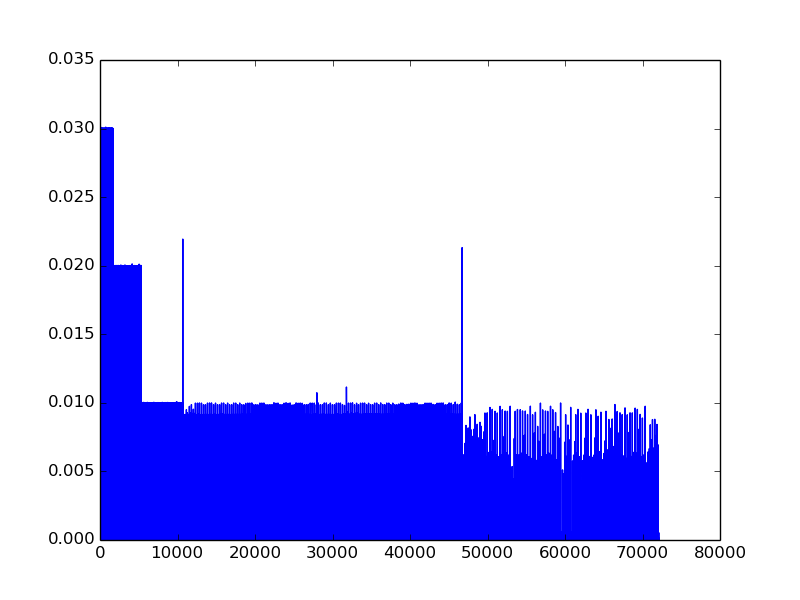
\includegraphics[width=0.5\textwidth]{seconds_http.png}
\caption{Zeit in Sekunden für je 1000 Byte}
\end{figure}
\end{frame}

\begin{frame}
\frametitle{FTP Server Ergebnisse}
\begin{itemize}
\item Drosselung am Ende des Downloads
\end{itemize}
\begin{figure}
\centering
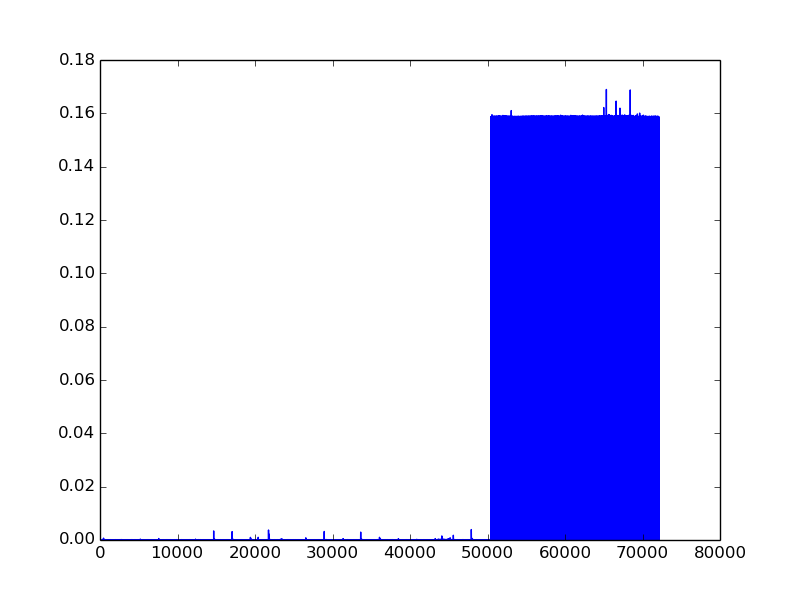
\includegraphics[width=0.5\textwidth]{seconds_ftp.png}
\caption{Zeit in Sekunden für je 1000 Byte}
\end{figure}
\end{frame}

\end{document}